\documentclass[11pt,a4paper]{article}

% ------------------------------------------------------------
% Multi-Agent Systems and Agentic AI practical examination
% LaTeX report template
% ------------------------------------------------------------
% Required format from coursework brief:
% - A4 paper
% - 11 pt body font
% - Single column
% - Margins of at least 2 cm
% - Single line spacing
% - Single PDF covering both parts
% - Section I.4 must be typeset in LaTeX
% - Every URL must be clickable
% ------------------------------------------------------------

\usepackage[a4paper,margin=2cm]{geometry}
\usepackage{setspace}
\singlespacing

\usepackage[T1]{fontenc}
\usepackage[utf8]{inputenc}
\usepackage{lmodern}
\usepackage[british]{babel}
\usepackage{microtype}

\usepackage{amsmath,amssymb,mathtools,bm}
\usepackage{graphicx}
\usepackage{booktabs}
\usepackage{array}
\usepackage{enumitem}
\usepackage{xcolor}
\usepackage{caption}
\usepackage{subcaption}
\usepackage{float}
\usepackage{tikz}
\usetikzlibrary{arrows.meta,positioning,shapes.geometric,fit}

\usepackage[hidelinks]{hyperref}
\usepackage[nameinlink,noabbrev]{cleveref}

% ------------------------------------------------------------
% Helpful commands
% ------------------------------------------------------------
\newcommand{\code}[1]{\texttt{#1}}
\newcommand{\repo}{\href{https://gitlab.developers.cam.ac.uk/YOUR-CRSID/YOUR-REPO}{GitLab repository}}
\newcommand{\wandb}{\href{https://wandb.ai/YOUR-PROJECT/YOUR-RUN}{W\&B run}}
\newcommand{\cmbcommit}{\href{https://github.com/borisbolliet/cmbagent_lg/tree/d7d0592a714e4cc01c97f1b77afdd57a208b18db}{\code{cmbagent\_lg}}}
\newcommand{\TODO}[1]{\textcolor{red}{[TODO: #1]}}

\setlist[itemize]{leftmargin=*,topsep=2pt,itemsep=1pt}
\setlist[enumerate]{leftmargin=*,topsep=2pt,itemsep=1pt}

% Keep tables compact by default
\renewcommand{\arraystretch}{1.12}

% ------------------------------------------------------------
% Metadata
% ------------------------------------------------------------
\title{Multi-Agent Systems and Agentic AI\\Practical Examination Report}
\author{Frederick Lawrence \\ CRSid: fl482 \\ Team members for Part I: Baron Gracias, Harvey Bermingham}
\date{\today}

\begin{document}

\maketitle

\noindent\textbf{Repository and logs.}
The code used for Part I is available at \repo. Training and evaluation logs are available at \wandb. The adaptive-planning implementation studied in Part II is linked at \cmbcommit. Replace the Part I placeholders with exact clickable URLs.

\vspace{0.5em}
\noindent\textbf{Notes on jointly owned work.}
Sections I.1--I.3 describe experiments run using the shared team TPU and shared repository. The analysis and prose in this report are my own. Section I.4 and Part II are completed individually.

\tableofcontents
\newpage

% ============================================================
\section*{Part I: GRPO finetuning of Gemma 3 on a TPU}
\addcontentsline{toc}{section}{Part I: GRPO finetuning of Gemma 3 on a TPU}
% Sections I.1--I.3 together should be at most 3 pages, excluding references and appendix.
% I.4 has no page limit, but should be clear and concise.

\subsection*{I.1 Reproducing the baseline}
\addcontentsline{toc}{subsection}{I.1 Reproducing the baseline}

\paragraph{Run details.}
\begin{table}[H]
    \centering
    \caption{Baseline run details.}
    \label{tab:baseline-run-details}
    \begin{tabular}{ll}
        \toprule
        Item & Value \\
        \midrule
        Repository commit & \code{TODO} \\
        TPU type & v6e-1 \\
        Training command & \code{python scripts/train.py} \\
        Evaluation command & \code{python scripts/evaluate.py} \\
        Wall-clock time & \TODO{e.g. 6 h 20 min} \\
        GRPO steps completed & \TODO{number of steps} \\
        Held-out split & \TODO{e.g. GSM8K test split} \\
        Evaluation seed & \TODO{fixed seed} \\
        \bottomrule
    \end{tabular}
\end{table}

\paragraph{Baseline patches.}
\TODO{State whether the baseline ran as shipped. If not, document the minimal fix required, with the affected file and commit. Keep this short.}

\paragraph{Evaluation.}
\begin{table}[H]
    \centering
    \caption{Baseline GSM8K accuracy.}
    \label{tab:baseline-accuracy}
    \begin{tabular}{lccc}
        \toprule
        Model & Split & Seed & Accuracy \\
        \midrule
        Base model, \code{google/gemma-3-1b-it} & \TODO{split} & \TODO{seed} & \TODO{value} \\
        LoRA GRPO checkpoint & \TODO{split} & \TODO{seed} & \TODO{value} \\
        \bottomrule
    \end{tabular}
\end{table}

\begin{figure}[H]
    \centering
    \includegraphics[width=0.82\linewidth]{figures/baseline_reward_kl.pdf}
    \caption{Baseline training curves showing mean reward $\bar r$ and $\mathrm{KL}(\pi_\theta\|\pi_{\mathrm{ref}})$ against GRPO step.}
    \label{fig:baseline-reward-kl}
\end{figure}

\subsection*{I.2 Understanding the baseline}
\addcontentsline{toc}{subsection}{I.2 Understanding the baseline}
% This subsection should be at most one page.

\paragraph{Policies in the LoRA setup.}
\TODO{Explain what plays the role of $\pi_\theta$, $\pi_{\mathrm{old}}$ and $\pi_{\mathrm{ref}}$, and identify which carries trainable parameters.}

\paragraph{Group size and advantage estimator.}
\TODO{State the group size $K$ from \code{scripts/config.py}. Identify the Tunix advantage estimator and state whether it is standard group-mean or leave-one-out.}

\paragraph{Reward terms.}
\TODO{Identify shaping rewards and the true correctness reward in \code{scripts/rewards.py}. Explain what would happen early in training with correctness reward alone in terms of within-group reward variance $\sigma_r$.}

\paragraph{Clipped surrogate.}
\TODO{Locate where the PPO-style clipped surrogate is implemented in Tunix. State what $\varepsilon$ corresponds to in \code{scripts/config.py} and note any deviation from the lecture form, such as per-token rather than per-sequence ratios.}

\subsection*{I.3 Improving on the baseline}
\addcontentsline{toc}{subsection}{I.3 Improving on the baseline}

\paragraph{Modification and motivation.}
\TODO{Describe the principled modification. Examples: leave-one-out advantage, sweep $K$, change $\beta$ or $\varepsilon$, modify shaping rewards, add length penalty, change LoRA rank, learning rate, schedule or generation length. Connect the choice to GRPO theory.}

\paragraph{Controlled comparison.}
\TODO{State how the comparison was controlled: same data, same evaluation split, same total compute or normalised per step. Mention baseline plus at least two further complete runs, or justify fewer.}

\begin{table}[H]
    \centering
    \caption{Controlled comparison on held-out GSM8K. Include uncertainty using a second seed or a bootstrap confidence interval over evaluation prompts.}
    \label{tab:controlled-comparison}
    \begin{tabular}{lcccc}
        \toprule
        Model / run & Modification & Seed(s) & Accuracy & Uncertainty \\
        \midrule
        Base model & None & \TODO{} & \TODO{} & \TODO{} \\
        Baseline GRPO & Default config & \TODO{} & \TODO{} & \TODO{} \\
        Variant 1 & \TODO{} & \TODO{} & \TODO{} & \TODO{} \\
        Variant 2 & \TODO{} & \TODO{} & \TODO{} & \TODO{} \\
        \bottomrule
    \end{tabular}
\end{table}

\begin{figure}[H]
    \centering
    \includegraphics[width=0.82\linewidth]{figures/reward_kl_variants.pdf}
    \caption{Training curves for the baseline and variants on shared axes, showing mean reward and KL over GRPO step.}
    \label{fig:reward-kl-variants}
\end{figure}

\begin{figure}[H]
    \centering
    \includegraphics[width=0.82\linewidth]{figures/grpo_diagnostic.pdf}
    \caption{Diagnostic plot for a known GRPO failure mode, such as advantage distribution, degenerate reward groups, response length, entropy, or KL versus accuracy.}
    \label{fig:grpo-diagnostic}
\end{figure}

\paragraph{Discussion.}
\TODO{Connect the empirical findings to lecture theory. State whether the observed behaviour matched the prediction, and diagnose any negative results honestly.}

\subsection*{I.4 GRPO theory}
\addcontentsline{toc}{subsection}{I.4 GRPO theory}
% This section must be written in LaTeX. There is no page limit, but verbosity is penalised.
% Use amsmath environments and number equations that you refer back to.

\subsubsection*{Question 1}
\addcontentsline{toc}{subsubsection}{Question 1}

\paragraph{(i)}
Since $\mathbb{E}[\bar r]=\mu$,
\[
    \mathbb{E}[\hat A_i]
    = \frac{\mathbb{E}[r_i]-\mathbb{E}[\bar r]}{\sigma}=0,
    \qquad
    \mathbb{E}[X_i]=h_i\mathbb{E}[\hat A_i]=0,
    \qquad
    \mathbb{E}[\hat g]
    =\frac{1}{K}\sum_{i=1}^{K}\mathbb{E}[X_i]=0.
\]
This expectation averages only reward noise around fixed completions. GRPO is an on-policy method so the completions are sampled from the policy, and the score gradient $\nabla_\theta\log\pi_\theta(a\mid q)$ can be correlated with the reward of the sampled completion and the policy gradient does not vanish.

\paragraph{(ii)}
The common random term is the group mean $\bar r$, which appears in every advantage:
\[
    X_i=h_i\hat A_i=\frac{h_i}{\sigma}(r_i-\bar r).
\]
For $i\ne j$,
\begin{align*}
    \operatorname{Cov}(X_i,X_j)
    &=\frac{h_i h_j^\top}{\sigma^2}
      \operatorname{Cov}(r_i-\bar r,r_j-\bar r),\\
    \operatorname{Cov}(r_i-\bar r,r_j-\bar r)
    &=0-\frac{\sigma^2}{K}-\frac{\sigma^2}{K}
      +\frac{\sigma^2}{K}
      =-\frac{\sigma^2}{K}.
\end{align*}
Therefore
\[
    \boxed{
        \operatorname{Cov}(X_i,X_j)=-\frac{1}{K}h_i h_j^\top,
        \qquad i\ne j.
    }
\]
The negative sign is the result of using a group centred contrast: if one completion is above the group mean, the others are pushed below that same mean.  This removes prompt-level reward offsets in GRPO, but the $K$ rollouts are no longer independent samples.

\paragraph{(iii)}
The naive i.i.d.\ calculation would instead treat the \(X_i\) as independent copies of \(X_1\), giving
\[
    \operatorname{Var}_{\mathrm{iid}}(\hat g)
    =
    \frac{1}{K}\operatorname{Var}(X_1)
    =
    \frac{K-1}{K^2}h_1h_1^\top .
\]
The discrepancy is that the true variance depends on the empirical spread of the score vectors around their group mean:
\[
    \operatorname{Var}(\hat g)
    =
    \frac{1}{K^2}\sum_i(h_i-\bar h)(h_i-\bar h)^\top .
\]
Thus the effective sample size should be defined by matching the variance of the actual estimator to an i.i.d.\ estimator.  In any direction \(u\),
\[
    u^\top \operatorname{Var}(\hat g)u
    =
    \frac{1}{K_{\mathrm{eff}}(u)}
    u^\top\operatorname{Var}(X_1)u,
\]
so
\[
    \boxed{
    K_{\mathrm{eff}}(u)
    =
    \frac{u^\top\operatorname{Var}(X_1)u}
         {u^\top\operatorname{Var}(\hat g)u}
    =
    \frac{\frac{K-1}{K}(u^\top h_1)^2}
         {\frac{1}{K^2}\sum_i\{u^\top(h_i-\bar h)\}^2}.
    }
\]
For diverse score directions, the denominator is typically \(O(1/K)\), so \(K_{\mathrm{eff}}\) grows roughly linearly with \(K\).  If all \(h_i\) are identical, then \(\sum_i \hat A_i=0\) makes \(\hat g=0\) exactly; more generally, if all \(h_i\) are aligned, only variation in their magnitudes contributes, so extra rollouts that produce the same update direction add little useful RL signal despite increasing sampling cost. 
% This is one of the reasons $K$ is typically kept small

\subsubsection*{Question 2}
\addcontentsline{toc}{subsubsection}{Question 2}

\paragraph{(i)}
Assuming $\pi_t(a)>0$ is on its support and with finite normalisation constant, any optimiser must have support contained in that of $\pi_t$ otherwise $\operatorname{KL}(\pi\Vert\pi_t)=\infty$.
With $\lambda$ enforcing $\sum_a\pi(a)=1$, stationarity gives
\[
    A_t(a)-\frac{1}{\eta}
       \left(\log\frac{\pi(a)}{\pi_t(a)}+1\right)+\lambda=0.
\]
Normalising the resulting exponential tilt yields the unique optimiser
\begin{equation}
    \pi_{t+1}(a)
    =\frac{\pi_t(a)\exp\{\eta A_t(a)\}}
           {Z_t},
    \qquad
    Z_t=\sum_b\pi_t(b)\exp\{\eta A_t(b)\}.
    \label{eq:q2-exp-update}
\end{equation}
The objective is strictly concave on this support, so the optimiser is
unique.  This is the KL mirror-descent or exponential-tilting update:
small $\eta$ gives a conservative RLHF step near $\pi_t$, while large
$\eta$ concentrates probability on high-advantage responses but cannot put
mass on responses assigned zero probability by $\pi_t$.

\paragraph{(ii)}
Let
$F_t(\pi)=\mathbb{E}_{a\sim\pi}[A^{\pi_t}(a)]
-\eta^{-1}\operatorname{KL}(\pi\Vert\pi_t)$.
The defining property of the true advantage is
$\mathbb{E}_{a\sim\pi_t}[A^{\pi_t}(a)]=0$, so $F_t(\pi_t)=0$.  Optimality
of \cref{eq:q2-exp-update} then implies
\[
    J(\pi_{t+1})
    =\mathbb{E}_{\pi_{t+1}}[A^{\pi_t}]
    \geq \frac{1}{\eta}\operatorname{KL}(\pi_{t+1}\Vert\pi_t)
    \geq 0
    =J(\pi_t).
\]
Thus the exact unrestricted update is monotone in this advantage objective.
In neural-network GRPO the exponential-tilted distribution may be outside
the model or LoRA-adapter family, and the advantage is a finite-sample,
group-normalised estimate.  Either approximation, especially with degenerate
groups where $\sigma_r$ is tiny or zero, can break the guarantee.

\paragraph{(iii)}
For $\hat A_t>0$, clipping removes the incentive to increase the sampled
ratio beyond $1+\varepsilon$; for $\hat A_t<0$, it removes the incentive to
decrease it below $1-\varepsilon$.  The resulting trust region is
advantage-dependent, samplewise, and soft: it clips the objective on sampled
actions, but does not enforce the ratio bounds after a shared neural update.
By contrast,
$\operatorname{KL}(\pi_\theta(\cdot\mid q)\Vert
\pi_{\mathrm{old}}(\cdot\mid q))\leq\delta$ is one hard,
distribution-level constraint; it can permit a large change on some actions
provided the joint KL budget remains satisfied.  In LLM RLHF this means PPO
clipping can miss unsampled completions and prompt-level KL spikes, whereas
a KL constraint directly budgets total distributional drift.

\subsubsection*{Question 3}
\addcontentsline{toc}{subsubsection}{Question 3}

\paragraph{(i)}
For any integrand $f$ where $\mathbb{E}_{\pi_{\mathrm{old}}}[f] =\mathbb{E}_{\pi_{\mathrm{mix}}}[wf]$, the importance weighing $w_i$ is
\begin{equation}
    w_i
    =\frac{\pi_{\mathrm{old}}(a_i\mid q)}
           {\pi_{\mathrm{mix}}(a_i\mid q)}
    =\frac{\pi_{\mathrm{old}}(a_i\mid q)}
           {(1-\alpha)\pi_{\mathrm{old}}(a_i\mid q)
             +\alpha\pi_{\mathrm{unif}}(a_i\mid q)}.
    \label{eq:q3-weight}
\end{equation}
Therefore, the importance-corrected gradient estimator $\hat g_{\mathrm{mix}}$ is 
\begin{equation}
    \hat g_{\mathrm{mix}}
    =\frac{1}{K}\sum_{i=1}^{K}
       w_i\nabla_\theta\log\pi_\theta(a_i\mid q)\,
       \frac{r_i-\bar r}{\sigma_r},
    \qquad a_i\overset{\mathrm{iid}}{\sim}\pi_{\mathrm{mix}}.
    \label{eq:q3-raw-mix}
\end{equation}

\paragraph{(ii)}
For each fixed realised action, $\pi_{\mathrm{mix}}(a_i\mid q)\to \pi_{\mathrm{old}}(a_i\mid q)$ and hence $w_i\to1$.  The realised $r_i$, $\bar r$, and $\sigma_r$ are unchanged, so \cref{eq:q3-raw-mix} tends to $\hat g_{\mathrm{GRPO}}$.

\paragraph{(iii)}
Linearity of expectation gives
\[
    V^{\pi_{\mathrm{mix}}}(q)
    =(1-\alpha)V^{\pi_{\mathrm{old}}}(q)
      +\alpha V^{\pi_{\mathrm{unif}}}(q).
\]
Consequently, multiplying by $w_i$ outside the advantage does not change the fact that the unweighted $\bar r$ estimates $V^{\pi_{\mathrm{mix}}}$ rather than $V^{\pi_{\mathrm{old}}}$.  For the fixed-scale target $\mathbb{E}_{\pi_{\mathrm{old}}}[ \nabla_\theta\log\pi_\theta(a\mid q)(R(q,a) V^{\pi_{\mathrm{old}}})/s]$ the leave-one-out (LOO) weighted baseline is needed.
\begin{equation}
    \hat V_{-i}
      =\frac{1}{K-1}\sum_{j\ne i}w_jr_j,
    \qquad
    \hat g_{\mathrm{mix}}^{\mathrm{LOO}}
      =\frac{1}{K}\sum_i
        w_i\nabla_\theta\log\pi_\theta(a_i\mid q)
        \frac{r_i-\hat V_{-i}}{s}.
    \label{eq:q3-loo-adv}
\end{equation}
$\mathbb{E}_{\pi_{\mathrm{mix}}}[\hat V_{-i}] =V^{\pi_{\mathrm{old}}}$ and $\hat V_{-i}$ is independent of $a_i$, so \cref{eq:q3-loo-adv} is unbiased for that old-policy score--advantage expectation. The common self-normalised baseline $\hat V_{\mathrm{SN}}=\sum_jw_jr_j/\sum_jw_j$ is often lower variance and consistent, but it is biased at finite $K$; using the same group's empirical $\sigma_r$ adds the usual GRPO normalisation bias and fails when the group reward variance is zero. Thus the reweighted LOO advantage is
\[
    \tilde A_i^{\mathrm{LOO}}
    =
    \frac{r_i-\hat V_{-i}}{s}.
\]

\paragraph{(iv)}
There are two variance effects.  First, the unweighted reward variance under the proposal is
\begin{align*}
    \operatorname{Var}_{\pi_{\mathrm{mix}}}(R)
    ={}&(1-\alpha)\operatorname{Var}_{\pi_{\mathrm{old}}}(R)
       +\alpha\operatorname{Var}_{\pi_{\mathrm{unif}}}(R)\\
      &+\alpha(1-\alpha)
        \bigl(V^{\pi_{\mathrm{old}}}-V^{\pi_{\mathrm{unif}}}\bigr)^2 .
\end{align*}
Thus mixing increases advantage variance when the uniform sampler has much larger reward variance or a very different mean, as with rare correct answers mixed with many invalid LLM completions.  It decreases raw advantage variance when $V^{\pi_{\mathrm{unif}}}\simeq V^{\pi_{\mathrm{old}}}$ and
$\operatorname{Var}_{\pi_{\mathrm{unif}}}(R)
<\operatorname{Var}_{\pi_{\mathrm{old}}}(R)$, for example if uniform
exploration smooths a spiky old-policy reward distribution.

Second, importance weighting changes the gradient estimator variance.  For a scalar projection $Y$ of the score--advantage term,
\[
    \mathbb{E}_{\pi_{\mathrm{mix}}}[w^2Y^2]
    =\mathbb{E}_{\pi_{\mathrm{old}}}[wY^2].
\]
Therefore lower raw reward variance does not guarantee lower gradient
variance: large-$|Y|$ samples in regions where
$\pi_{\mathrm{old}}>\pi_{\mathrm{mix}}$ get $w>1$ and can dominate, while adding proposal mass in regions that contribute substantially to the old-policy second moment can reduce variance by lowering their importance weights.

\paragraph{(v)}
Under the stated assumption,
\[
    w_i=c^T=\exp(T\log c)\longrightarrow0
    \quad\text{exponentially as }T\to\infty.
\]
When $\alpha>0$, mixture samples include tokens to which the uniform
component assigns more probability than $\pi_{\mathrm{old}}$; more formally,
$\mathbb{E}_{\pi_{\mathrm{mix}}}
[\log(\pi_{\mathrm{old}}/\pi_{\mathrm{mix}})]
=-\operatorname{KL}(\pi_{\mathrm{mix}}\Vert\pi_{\mathrm{old}})<0$, so the
geometrically typical token ratio is below one.  Consequently most long
responses have negligible weight while a few rare trajectories dominate,
which is disastrous for long-form LLM RLHF because the effective sample size
collapses exponentially with response length.  One concrete fix is to scale
the mixture coefficient as $\alpha=\gamma/T$, keeping the cumulative
proposal perturbation, and hence typical log-weight magnitude, $O(1)$; the
trade-off is weaker uniform exploration for longer responses.

% ============================================================
\section*{Part II: Adaptive planning in \cmbcommit}
\addcontentsline{toc}{section}{Part II: Adaptive planning in cmbagent\_lg}
% Part II should be at most 2 pages, excluding the workflow diagram.

\subsection*{II.1 Workflow diagram}
\addcontentsline{toc}{subsection}{II.1 Workflow diagram}

\begin{figure}[H]
    \centering
    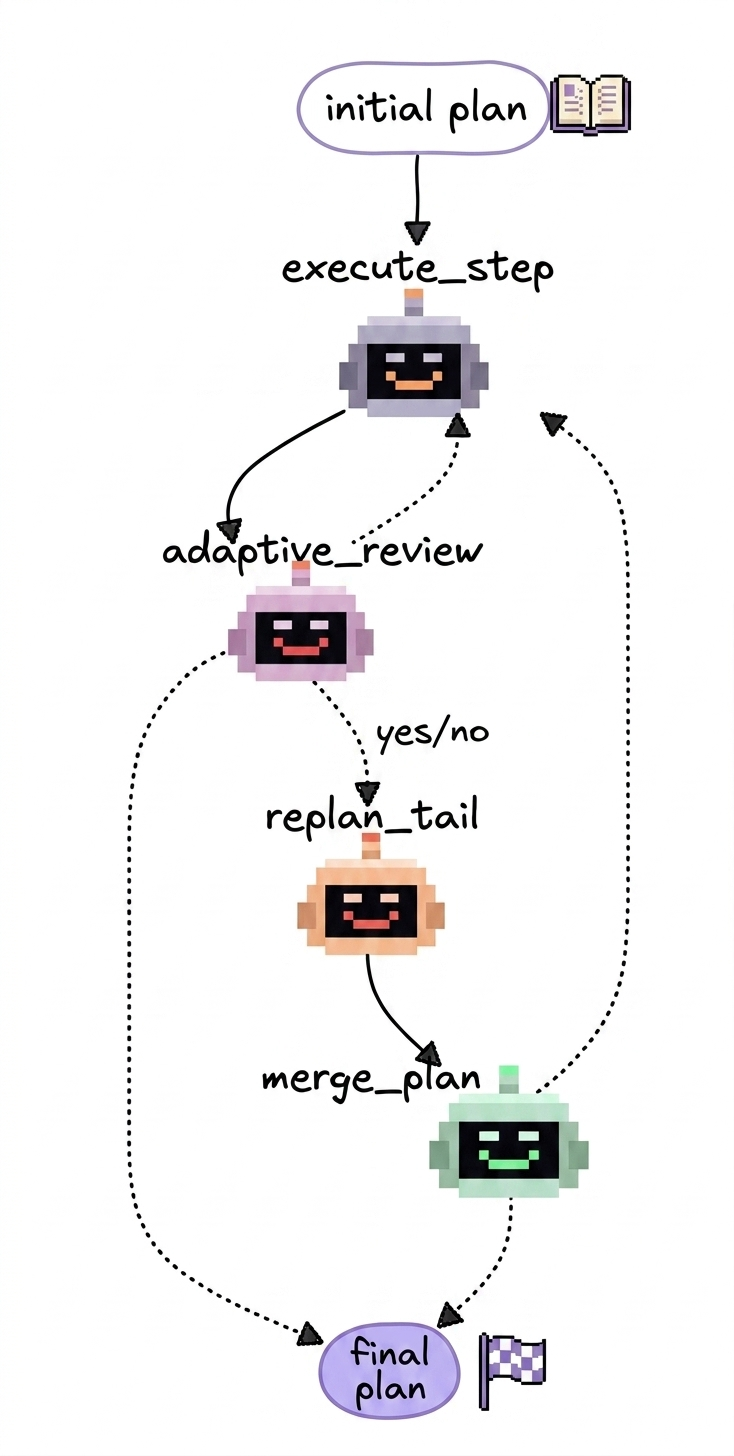
\includegraphics[width=0.95\linewidth,height=0.72\textheight,keepaspectratio]{figures/lg_diagram.jpg}
    \caption{Workflow diagram of the adaptive-planning graph in \cmbcommit. Dotted edges are conditional routes from the reviewer and merge routers; solid edges are unconditional graph transitions.}
    \label{fig:adaptive-planning-langgraph}
\end{figure}

% \begin{figure}[H]
%     \centering
%     \small
%     \resizebox{\linewidth}{!}{%
%     \begin{tikzpicture}[
%         node distance=0.9cm and 1.15cm,
%         box/.style={draw,rounded corners,align=center,minimum width=2.55cm,minimum height=0.78cm,font=\small},
%         widebox/.style={draw,rounded corners,align=center,minimum width=3.25cm,minimum height=0.78cm,font=\small},
%         decision/.style={draw,diamond,aspect=2.25,align=center,inner sep=1pt,font=\small},
%         statebox/.style={draw,dashed,rounded corners,align=left,font=\scriptsize,text width=0.89\linewidth,inner sep=4pt},
%         arrow/.style={-Latex,thick}
%     ]
%         \node[widebox] (plan) {initial planning graph\\planner $\leftrightarrow$ reviewer\\final \code{Plan}};
%         \node[box,right=of plan] (start) {START};
%         \node[widebox,right=of start] (exec) {\code{execute\_step}\\alias of\\\code{deep\_research.run\_step}};
%         \node[widebox,right=of exec] (review) {\code{adaptive\_review}\\LLM emits\\\code{AdaptiveReview}};
%         \node[decision,below=of review] (route) {\code{route\_after\_review}};
%         \node[widebox,left=of route] (replan) {\code{replan\_tail}\\rewrite remaining\\steps};
%         \node[widebox,left=of replan] (merge) {\code{merge\_plan}\\completed prefix\\+ new tail};
%         \node[box,right=of route] (end) {END};
%         \node[statebox,below=1.05cm of replan,anchor=north west,xshift=-1.4cm] (state) {
%             Threaded state: \code{plan}, \code{step\_index}, \code{step\_summaries}, \code{step\_outcomes}, \code{work\_dir}, \code{adaptive\_review}, \code{new\_tail}, \code{adaptive\_history}.\\
%             Run context: \code{PlanContext} with \code{main\_task}, model choices, \code{available\_agents}, and execution budgets.
%         };

%         \draw[arrow] (plan) -- (start);
%         \draw[arrow] (start) -- (exec);
%         \draw[arrow] (exec) -- (review);
%         \draw[arrow] (review) -- (route);
%         \draw[arrow] (route) -- node[above]{failed step or exhausted plan} (end);
%         \draw[arrow] (route) -- node[above]{\code{needs\_adaptation}} (replan);
%         \draw[arrow] (replan) -- (merge);
%         \draw[arrow] (merge.north) |- node[pos=0.23,above]{steps remain} (exec.south);
%         \draw[arrow] (route.south) -- ++(0,-0.42) -| node[pos=0.28,below]{no adaptation} (exec.south);
%         \draw[arrow] (merge.south) |- node[pos=0.22,below]{new plan exhausted} (end.south);
%     \end{tikzpicture}
%     }
%     \caption{Adaptive-planning workflow in \cmbcommit. The initial planner/reviewer loop produces the plan; the adaptive graph then executes one step at a time and may replace only the unexecuted tail. The diagram is excluded from the Part II page limit.}
%     \label{fig:adaptive-planning-workflow}
% \end{figure}

\paragraph{Walkthrough.}
I studied \cmbcommit.  The initial \code{planning} graph is open-loop: a planner and plan reviewer run a bounded propose--critique loop and produce a structured \code{Plan}.  The adaptive graph consumes that plan.  Its \code{execute\_step} node is the existing \code{deep\_research.run\_step}: it runs the current \code{Step}, appends a summary and outcome, checkpoints the deep-research run, and increments the 1-based \code{step\_index}.  After every executed step, \code{adaptive\_review} asks a critic model whether the remaining steps should be rewritten in light of the latest step summary and outcome.  The revision trigger is therefore the structured field \code{AdaptiveReview.needs\_adaptation}.  If it is true, \code{replan\_tail} asks the planner model for a replacement tail and \code{merge\_plan} splices \(\texttt{completed\_prefix}+\texttt{new\_tail}\) back into \code{plan}.  The completed prefix, its summaries, outcomes, and workspace artefacts are held fixed; only not-yet-executed steps may change.  The graph terminates when the latest step is unfulfilled, when \code{step\_index} is beyond the current plan length, or when a rewrite leaves no remaining steps.  Otherwise control returns to \code{execute\_step}.

\subsection*{II.2 Problems}
\addcontentsline{toc}{subsection}{II.2 Problems}

\paragraph{Problem 1: an informal feedback controller.}
The adaptive graph is closed-loop, but the feedback controller is weak.  As shown in \Cref{fig:adaptive-planning-langgraph}, the only trigger for replanning is the LLM-generated field \code{AdaptiveReview.needs\_adaptation}, computed from the latest step summary, latest outcome, and remaining tail.  There is no explicit uncertainty estimate, cost model, value-of-information test, or task-level error signal.  This means the system can observe execution feedback but cannot reliably decide whether rewriting the plan is worth the extra cost.  In practice, this can cause unnecessary replanning after harmless new information, or leave an invalid tail unchanged when the reviewer fails to recognise that the plan has become stale.
\TODO{manually review}

\paragraph{Problem 2: failures end the outer loop rather than trigger repair.}
If the code returns an error or fails to execute properly, the \code{adaptive\_review} agent will mark the step as unfulfilled and the loop will immediately end. During execution, the engineer agent can invoke the \code{self\_debug} loop but this targets bugs in the code rather than fundamental flaws in the plan. This is an issue because code failing to run is often one of the clearest pieces of evidence that the plan itself is wrong. It does not give the system the chance to review the error and rewrite dependent future steps. The result is a system that can adapt after successful steps, but is least adaptive when plan level recovery would be most useful.

\paragraph{Problem 3: tail rewrites are myopic and unvalidated.}
The initial planner uses a reviewer loop and keeps review history, whereas the adaptive replanner directly produces a new tail.  The reviewer sees the latest result and the remaining steps, but not the full initial planning transcript or a rich history of earlier adaptations.  After \code{replan\_tail}, \code{merge\_plan} splices the new tail into the plan without checking task coverage, dependencies on completed artefacts, plan length, or whether the recommendations were actually followed.  The dynamic schema prevents invalid agent names, but it does not ensure that the repaired plan is better.  This makes the adaptive update potentially destabilising: a weak rewrite can replace a sound remaining plan.  The risk is increased by the lack of a revision budget and by the thin \code{adaptive\_history}, which omits the old tail, new tail, and reviewer reason from the persisted evidence.
\TODO{manually review - no check that the tail is actually better}

\subsection*{II.3 Proposed improvements}
\addcontentsline{toc}{subsection}{II.3 Proposed improvements}

\paragraph{Structured adaptation policy.}
Extend \code{AdaptiveReview} with structured fields for reason category, confidence, expected benefit, extra steps, and estimated cost.  Route to \code{replan\_tail} only when an explicit policy is met, for example a high-confidence hard invalidation or expected benefit above a threshold.  This makes the controller auditable and reduces gratuitous replanning.  The trade-off is prompt and schema complexity, and the numerical scores would still be model judgements rather than calibrated measurements.

\paragraph{Failure-aware replanning path.}
Before ending on \code{fulfilled=False}, add a bounded failure-review route that gives the replanner the failed step, failure reason, completed summaries, and remaining tail.  It could insert a repair step, replace the failed step, or mark the failure unrecoverable.  This separates local retry from plan-level repair and better matches closed-loop planning, where failures are observations to condition on.  The trade-off is extra latency after failures and the danger of repeatedly trying to repair an impossible task, so it needs a small retry/revision budget.

\paragraph{Validated, budgeted tail replacement.}
\TODO{merge\_plan should validate the plan before merging (effectively same as adaptive review)}
Insert a \code{validate\_new\_tail} node before \code{merge\_plan}.  It should check that the new tail preserves global task coverage, uses only available agents, does not duplicate completed steps, respects a maximum plan length, and follows the reviewer's recommendations; invalid tails can be sent back to \code{replan\_tail} with feedback, bounded by a \code{PlanContext} revision budget.  Persist each revision with old tail, new tail, reviewer reason, model names, and timestamps.  This improves stability and auditability, at the cost of another critic call per adaptation, larger checkpoints, and some risk of rejecting a creative but useful repair.

% ============================================================
\newpage
\section*{References}
\addcontentsline{toc}{section}{References}
% References do not count towards the page limits.
% Replace this manual list with biblatex or BibTeX if preferred.

\begin{itemize}
    \item Hu, E. J. et al. (2021). \emph{LoRA: Low-Rank Adaptation of Large Language Models}. \url{https://arxiv.org/abs/2106.09685}
    \item Tunix documentation or source link used for GRPO implementation: \url{https://github.com/google/tunix}
    \item Exact \code{cmbagent\_lg} adaptive-planning commit studied: \url{https://github.com/borisbolliet/cmbagent_lg/tree/d7d0592a714e4cc01c97f1b77afdd57a208b18db}
\end{itemize}

\appendix
\section{Appendix}
% Appendices do not count towards the page limits but must not contain material essential to marking.

\subsection{Additional run details}
\TODO{Optional non-essential logs, extra tables, hyperparameter dumps, and supplementary figures.}

\end{document}
